
\subsection{Mi primer \textit{Kotlin}}
  Ahora que ya sabemos cómo crear paquetes, vamos a crear nuestro primer archivo \textit{Kotlin}.
  Para ello, haremos click derecho sobre el paquete que acabamos de crear y seleccionaremos
  \textit{New} \texttt{->} \textit{Kotlin File/Class} (\cref{fig:idea64_new_kotlin_file}), y en
  el dialogo que aparece crearemos un archivo \texttt{InteractiveFibonacciCalculator} 
  (\cref{fig:idea64_new_kotlin_file_dialog}).

  \begin{figure}[ht!]
    \centering
    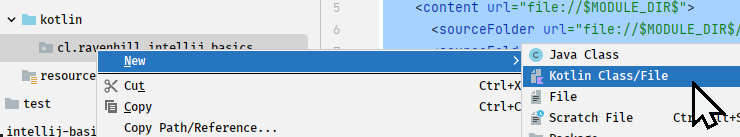
\includegraphics[width=0.8\textwidth]{img/Por_algo_se_empieza/idea64_new_kotlin_file.png}
    \caption{Creando un nuevo archivo \textit{Kotlin}}
    \label{fig:idea64_new_kotlin_file}
  \end{figure}

  \begin{figure}[H]
    \centering
    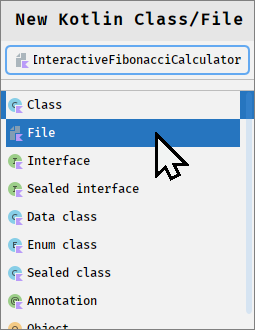
\includegraphics[width=0.3\textwidth]{img/Por_algo_se_empieza/idea64_new_kotlin_file_dialog.png}
    \caption{Creando un nuevo archivo \textit{Kotlin}}
    \label{fig:idea64_new_kotlin_file_dialog}
  \end{figure}

  Esto creará un archivo \texttt{InteractiveFibonacciCalculator.kt} en la carpeta
  \url{src/main/kotlin/cl/ravenhill/intellij/basics}.
  Noten que el nombre del archivo utiliza \idxit{PascalCase}.\autocite{WhatPascalCase}

  Ahora vamos a escribir el código que calcula la sucesión de Fibonacci de forma interactiva.
  Lo primero que debemos conocer aquí es la función \texttt{main}.
  Esta función es el punto de entrada, es decir, es la función que se ejecuta cuando se corre el
  programa.

  Existe más de una forma de escribir la función \texttt{main} en \textit{Kotlin}, pero 
  utilizaremos la más simple, que es definir una función \texttt{main(): Unit}.
  Podemos partir con algo como:

  \begin{kotlin}
    package cl.ravenhill.intellij.basics

    fun main(): Unit {
      println("Welcome to the Fibonacci Calculator!")
    }
  \end{kotlin}

  ¡Y listo! 
  Tenemos nuestra primera aplicación en \textit{Kotlin}.
  Para ejecutarla, buscaremos el botón \textit{Run} ubicado al lado izquierdo de la declaración de 
  la función \texttt{main} (\cref{fig:idea64_run_button}), le daremos click y, en la pestaña que
  se abre, seleccionaremos \textit{Run `InteractiveFibonacci...'} (las otras opciones las 
  ignoraremos por ahora).

  \begin{figure}[ht!]
    \centering
    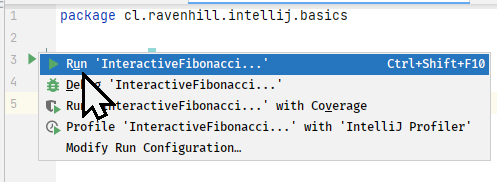
\includegraphics[width=0.5\textwidth]{img/Por_algo_se_empieza/idea64_run_button.png}
    \caption{Ejecutando la aplicación}
    \label{fig:idea64_run_button}
  \end{figure}